\documentclass[11pt]{article}
\usepackage[margin=1in]{geometry}
\usepackage{amsmath}
\usepackage{graphicx}
\usepackage{caption}
\usepackage{subcaption}
\usepackage{booktabs}
\usepackage{dcolumn}
\usepackage{float}

\newcolumntype{d}[1]{D{.}{.}{#1}}

\title{STAT 330 Final Project:\\Predicting House Prices in King County}
\author{Isabella Moreau \and Kwame Mensah}
\date{December 2026}

\begin{document}
\maketitle

\section{Introduction}
We model the sale price of 21\,613 homes sold in King County, Washington, between May
2014 and May 2015, using ordinary least squares on the log price.

\section{Exploratory analysis}
Figure~\ref{fig:eda} shows the distribution of prices and the relationship between living
area and price. Panel~\subref{fig:eda-b} suggests a log transformation.

\begin{figure}[H]
  \centering
  \begin{subfigure}[b]{0.45\textwidth}
    \centering
    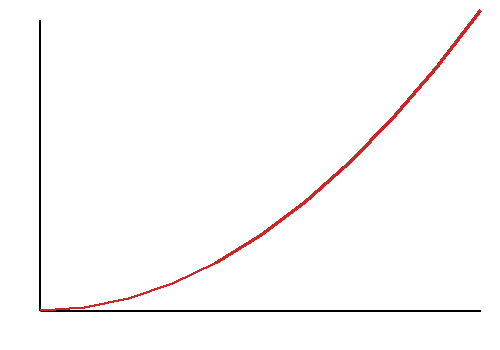
\includegraphics[width=\textwidth]{plot.png}
    \caption{Histogram of sale price.}
    \label{fig:eda-a}
  \end{subfigure}
  \hfill
  \begin{subfigure}[b]{0.45\textwidth}
    \centering
    
\includegraphics[width=\textwidth]{blocks.png}
    \caption{Price against living area.}
    \label{fig:eda-b}
  \end{subfigure}
  \caption{Exploratory plots.}
  \label{fig:eda}
\end{figure}

\section{Model}
\begin{equation}
\log(\text{price}_i) = \beta_0 + \beta_1\log(\text{sqft}_i) + \beta_2\,\text{grade}_i
  + \beta_3\,\text{waterfront}_i + \varepsilon_i,
  \qquad \varepsilon_i \sim \mathcal{N}(0,\sigma^2).
\end{equation}

\section{Results}
\begin{table}[H]
\centering
\caption{OLS estimates (dependent variable: log price).}
\label{tab:ols}
\begin{tabular}{l d{3.3} d{1.3} d{3.1}}
\toprule
\multicolumn{1}{c}{Variable} & \multicolumn{1}{c}{Estimate} &
\multicolumn{1}{c}{Std.\ error} & \multicolumn{1}{c}{$t$} \\
\midrule
Intercept      & 7.112  & 0.061 & 116.6 \\
log(sqft)      & 0.548  & 0.009 & 60.9 \\
Grade          & 0.187  & 0.003 & 62.3 \\
Waterfront     & 0.621  & 0.031 & 20.0 \\
\midrule
$R^2$          & 0.583  &       &       \\
$n$            & \multicolumn{1}{c}{21\,613} & & \\
\bottomrule
\end{tabular}
\end{table}

A 1\% increase in living area is associated with a 0.55\% increase in price, holding
grade and waterfront status fixed.

\section{Diagnostics}
Residual plots show mild heteroscedasticity; robust standard errors change none of our
conclusions.

\end{document}
